\documentclass[8pt]{beamer}

\usetheme{Madrid}

\usepackage[orientation=portrait,size=a1,scale=1]{beamerposter}
\usepackage[overlay]{textpos}

\usepackage[utf8]{inputenc}
\usepackage{default}
\usepackage{changepage}
\usepackage{subfigure}
\usepackage{graphicx}
\usepackage[sort&compress,comma,super]{natbib}
\usepackage[labelformat=empty]{caption}

\setlength{\columnsep}{5cm}
\setlength\labelsep{\dimexpr\labelsep + 0.6em\relax}  

\newlength{\wideitemsep}
\setlength{\wideitemsep}{\itemsep}
\addtolength{\wideitemsep}{10pt}
\let\olditem\item
\renewcommand{\item}{\setlength{\itemsep}{\wideitemsep}\olditem}

\usepackage{tikz}
\usetikzlibrary{calc}
\tikzset{egrid/.style={draw,help lines}}
\tikzset{mgrid/.style={draw,help lines,dashed}}
\tikzset{epoint/.style={draw,circle,red,inner sep=2pt,fill}}
\tikzset{mpoint/.style={draw,circle,blue,inner sep=2pt,fill}}

\definecolor{dark}{RGB}{0,105,0}

\setbeamertemplate{background canvas}[vertical shading][top=yellow!80!dark,bottom=yellow!60!dark]
\beamertemplatenavigationsymbolsempty
\setbeamertemplate{blocks}[rounded][shadow=false]
\setbeamercolor{block body}{bg=yellow!30}
\setbeamercolor{block title}{bg=dark}
\setbeamercolor{item}{fg=dark}
\setbeamertemplate{footline}{}

\title{Modelling light propagation through\\radial-director liquid crystal waveguides}

\author{\underline{Miha \v Can\v cula\inst{1}}\and Miha Ravnik\inst{1,2}\and Slobodan \v Zumer\inst{1,2,3}}
\institute{\inst{1}Faculty of Mathematics and Physics, University of Ljubljana, Slovenia\and\inst{2}Centre of excellence NAMASTE, Ljubljana, Slovenia\and\inst{3}Jo\v zef Stefan Institute, Ljubljana, Slovenia}

\newcommand{\blockpadding}{
  \rule[-0.6ex]{0pt}{2.5ex}
}

\addtobeamertemplate{block begin}
  {\vspace{1ex}}
  {\vspace{1ex} % Pads top of block
     % separates paragraphs in a block
   \setlength{\parskip}{24pt plus 1pt minus 1pt}%
   \begin{adjustwidth}{5mm}{5mm}
}
\addtobeamertemplate{block end}
  {\end{adjustwidth}%
   \vspace{1ex}}% Pads bottom of block
  {} % Seperates blocks from each other

\begin{document}

\begin{columns}
 \begin{column}{.976\textwidth}
  \begin{block}{}
\vspace{0.5cm}
\centering
{\fontsize{80}{96}\selectfont \inserttitle} \\
\vspace{1cm}
{\LARGE \underline{Miha \v Can\v cula$^{1}$}, Miha Ravnik$^{1,2}$, Slobodan \v Zumer$^{1,2,3}$} \\
\vspace{1cm}
{\large
$^{1}$Faculty of Mathematics and Physics, University of Ljubljana, Slovenia\\
$^{2}$Centre of excellence NAMASTE, Ljubljana, Slovenia \\
$^{3}$Jo\v zef Stefan Institute, Ljubljana, Slovenia
}
\vspace{0.5cm}
\end{block}


 \end{column}
\end{columns}
\begin{columns}[t]
 \begin{column}{.36\textwidth}
\begin{block}{\blockpadding Motivation}
\begin{itemize}
 \item Light guiding is central in complex optics and photonics, for example for efficient data transfer
 \item Combined birefringence and response to external stimuli in liquid crystal structures could be used for directed guiding of light -- such as in waveguides\citep{lasers}.
 \item Smectic A fibres with radial director profile can be created using 8CB and a surfactant
 \item Point defect in a nematic droplet turns a Gaussian beam into Laguerre-Gaussian\citep{brasselet} -- is there a similar effect caused by the line defect in a fibre?
\end{itemize}
\end{block}

\begin{block}{\blockpadding Methods}
 \begin{itemize}
  \item FDTD method\citep{taflove} -- direct time evolution of electromagnetic fields in 3D with fully anisotropic $\varepsilon$
  \item Assumed zero conductivity and empty space permeability in bulk.
  \item Simulate long cylindrical waveguide with periodic boundary conditions in $z$ direction
  \item Staggered grid, adapted for dielectric anisotropy
  \begin{figure}[h]
\centering
 \subfigure{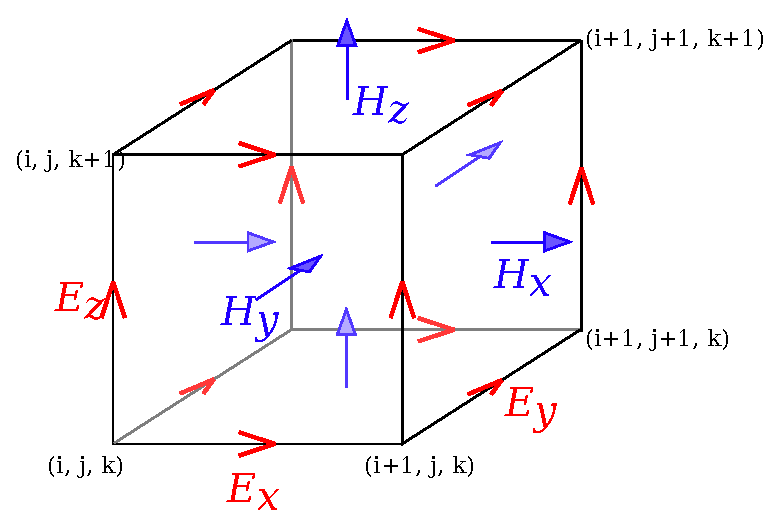
\includegraphics[width=.4\textwidth]{../Magisterij/Slike/Yee-cube}}
 \subfigure{\begin{tikzpicture}[scale=1.4]
    
    \foreach \x in {0,1}{
      \foreach \y in {0,1}{
        \node[mpoint] at (2*\x,2*\y) {}; 
        \node[mpoint] at (2*\x+1.2,2*\y+0.8) {}; 
        \node[epoint] at (2*\x+1.6,2*\y+1.4) {};
        \node[epoint] at (2*\x+1.6-1.2,2*\y+1.4-0.8) {};
        \draw[mgrid] (2*\x,2*\y) -- (2*\x+1.2,2*\y+0.8);
        \draw[egrid] (2*\x+1.6,2*\y+1.4) -- (2*\x+1.6-1.2,2*\y+1.4-0.8);
      }
    }
    
    \draw[mgrid] (0,0) rectangle (2,2);
    \draw[mgrid] (1.2,0.8) rectangle (3.2,2.8);
    \draw[egrid] (1.6,1.4) rectangle (3.6,3.4);
    \draw[egrid] (1.6-1.2,1.4-0.8) rectangle (3.6-1.2,3.4-0.8);
\end{tikzpicture}}
\label{fig:lattice}
\caption{{\color{dark} Left:} Yee lattice, optimized for diagonal dielectric tensor. \\{\color{dark} Right:} The lattice we used, suitable for full anisotropic $\varepsilon$. \\In both cases $\vec E$ and $\vec H$ are known at different times}
\end{figure}
  \item Tested with uniform director, refraction on interfaces, and periodic modulation of refraction index
  \vspace{-2ex}
  \begin{figure}[h]
   \centering
   \subfigure{\scalebox{0.77}{% GNUPLOT: LaTeX picture with Postscript
\begingroup
  \makeatletter
  \providecommand\color[2][]{%
    \GenericError{(gnuplot) \space\space\space\@spaces}{%
      Package color not loaded in conjunction with
      terminal option `colourtext'%
    }{See the gnuplot documentation for explanation.%
    }{Either use 'blacktext' in gnuplot or load the package
      color.sty in LaTeX.}%
    \renewcommand\color[2][]{}%
  }%
  \providecommand\includegraphics[2][]{%
    \GenericError{(gnuplot) \space\space\space\@spaces}{%
      Package graphicx or graphics not loaded%
    }{See the gnuplot documentation for explanation.%
    }{The gnuplot epslatex terminal needs graphicx.sty or graphics.sty.}%
    \renewcommand\includegraphics[2][]{}%
  }%
  \providecommand\rotatebox[2]{#2}%
  \@ifundefined{ifGPcolor}{%
    \newif\ifGPcolor
    \GPcolortrue
  }{}%
  \@ifundefined{ifGPblacktext}{%
    \newif\ifGPblacktext
    \GPblacktexttrue
  }{}%
  % define a \g@addto@macro without @ in the name:
  \let\gplgaddtomacro\g@addto@macro
  % define empty templates for all commands taking text:
  \gdef\gplbacktext{}%
  \gdef\gplfronttext{}%
  \makeatother
  \ifGPblacktext
    % no textcolor at all
    \def\colorrgb#1{}%
    \def\colorgray#1{}%
  \else
    % gray or color?
    \ifGPcolor
      \def\colorrgb#1{\color[rgb]{#1}}%
      \def\colorgray#1{\color[gray]{#1}}%
      \expandafter\def\csname LTw\endcsname{\color{white}}%
      \expandafter\def\csname LTb\endcsname{\color{black}}%
      \expandafter\def\csname LTa\endcsname{\color{black}}%
      \expandafter\def\csname LT0\endcsname{\color[rgb]{1,0,0}}%
      \expandafter\def\csname LT1\endcsname{\color[rgb]{0,1,0}}%
      \expandafter\def\csname LT2\endcsname{\color[rgb]{0,0,1}}%
      \expandafter\def\csname LT3\endcsname{\color[rgb]{1,0,1}}%
      \expandafter\def\csname LT4\endcsname{\color[rgb]{0,1,1}}%
      \expandafter\def\csname LT5\endcsname{\color[rgb]{1,1,0}}%
      \expandafter\def\csname LT6\endcsname{\color[rgb]{0,0,0}}%
      \expandafter\def\csname LT7\endcsname{\color[rgb]{1,0.3,0}}%
      \expandafter\def\csname LT8\endcsname{\color[rgb]{0.5,0.5,0.5}}%
    \else
      % gray
      \def\colorrgb#1{\color{black}}%
      \def\colorgray#1{\color[gray]{#1}}%
      \expandafter\def\csname LTw\endcsname{\color{white}}%
      \expandafter\def\csname LTb\endcsname{\color{black}}%
      \expandafter\def\csname LTa\endcsname{\color{black}}%
      \expandafter\def\csname LT0\endcsname{\color{black}}%
      \expandafter\def\csname LT1\endcsname{\color{black}}%
      \expandafter\def\csname LT2\endcsname{\color{black}}%
      \expandafter\def\csname LT3\endcsname{\color{black}}%
      \expandafter\def\csname LT4\endcsname{\color{black}}%
      \expandafter\def\csname LT5\endcsname{\color{black}}%
      \expandafter\def\csname LT6\endcsname{\color{black}}%
      \expandafter\def\csname LT7\endcsname{\color{black}}%
      \expandafter\def\csname LT8\endcsname{\color{black}}%
    \fi
  \fi
  \setlength{\unitlength}{0.0500bp}%
  \begin{picture}(7200.00,5040.00)%
    \gplgaddtomacro\gplbacktext{%
    }%
    \gplgaddtomacro\gplfronttext{%
      \csname LTb\endcsname%
      \put(3600,470){\makebox(0,0){\strut{}\footnotesize $z$}}%
      \put(932,2630){\rotatebox{-270}{\makebox(0,0){\strut{}\footnotesize $x$}}}%
    }%
    \gplbacktext
    \put(0,0){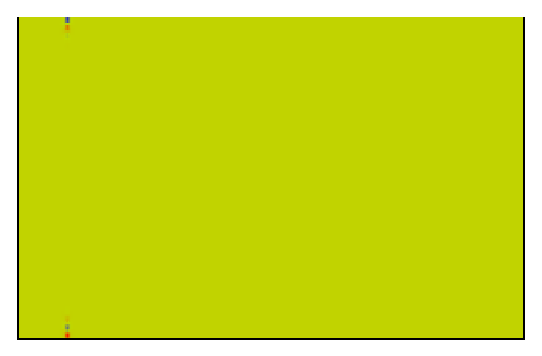
\includegraphics{/home/miha/Sola/Poster/refraction.eps}}%
    \gplfronttext
  \end{picture}%
\endgroup
}}
   \subfigure{\scalebox{0.7}{\input{g_test_uniform.tex}}}
   \caption{{\color{dark} Left:} Refraction on an interface near Brewster's angle. \\{\color{dark} Right:} Intensity of light transimitted through a uniform-director liquid crystal between crossed polarizers}
  \end{figure}
  \vspace{-2ex}
    \end{itemize}
  \end{block}
  
  \begin{block}{\blockpadding Parameters}
  \begin{itemize}
  \item Observe propagation of Gaussian laser pulse

\item Cylindrical waveguide with a radial director profile and a singular disclination line along its axis \\
\begin{figure}[h]
\centering
\subfigure{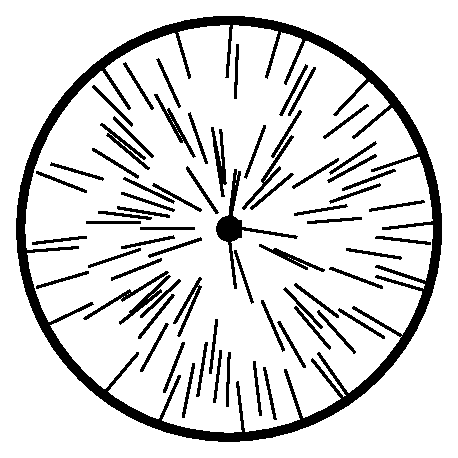
\includegraphics[height=.2\textwidth]{radial-cross}}
\subfigure{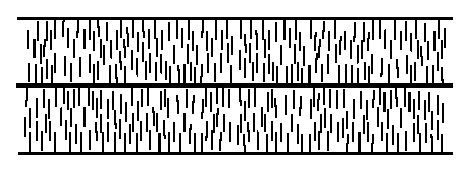
\includegraphics[height=.2\textwidth]{../Magisterij/Slike/director-profile-radial}}
\end{figure}
The core radius of the central +1 disclination line is much smaller than the wavelength and can therefore be neglected. 
\item Waveguide radius $5 - 20$ $\mu$m, inside 8CB with $n_o = 1.51$ and $n_e = 1.68$, surrounded by water with $n = 1.33$
\item Mesh size $512 \times 512 \times 256$.

 \end{itemize}
 \end{block}


 \end{column}
 
 \begin{column}{0.596\textwidth}
  \begin{block}{\blockpadding Electric field}
  \begin{itemize}
   \item A Gaussian beam entering a fibre turns into a Laguerre-Gaussian beam
   \item The difference in refraction index deforms the beam
   \vspace{1ex}
\begin{figure}[h]
\centering
 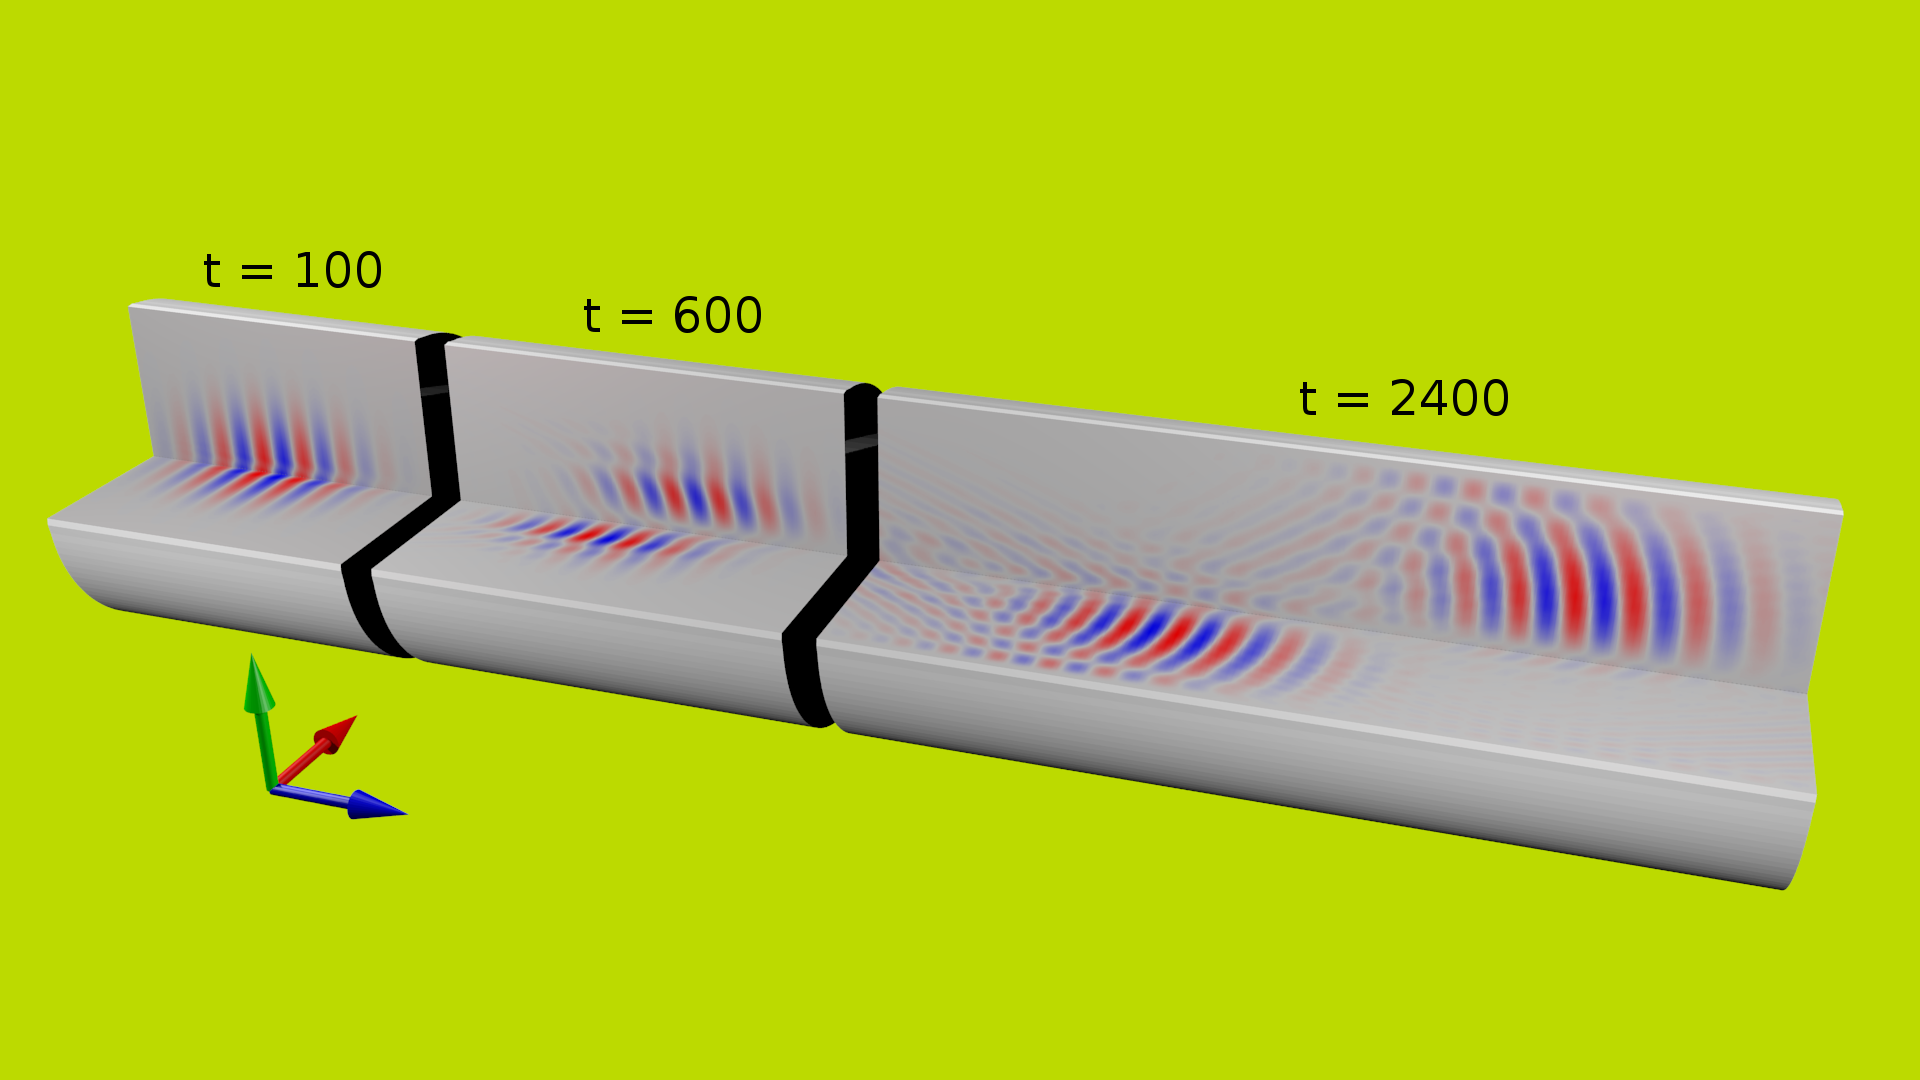
\includegraphics[width=.825\textwidth,clip,trim=0mm 50mm 0mm 80mm]{./render_t}
 \caption{Snapshots of electric field $\vec E$ at three different times. Incident light is polarized along the $x$ axis (red arrow). \\{\color{dark} Left:} The Gaussian pulse just after entering the waveguide. {\color{dark} Center:} After a short time, a dark spot forms near the axis. Regions near the $xz$ and $yz$ planes differ in propagation velocity and have opposite phase. {\color{dark} Right:} After a longer time, the difference in velocity greatly distorts the pulse. Reflection from waveguide walls causes noticeable interferrence and waveforms lose clarity, although the pattern remains visible. }
\end{figure}
\end{itemize}

\end{block}
\begin{block}{\blockpadding Pulse shape and polarization}
\begin{itemize}
\item The pulse deforms, then gradually splits into multiple intensity regions, positioned diagonally to the incident light polarization. 
\vspace{.3ex}
 \begin{figure}[h]
  \centering
  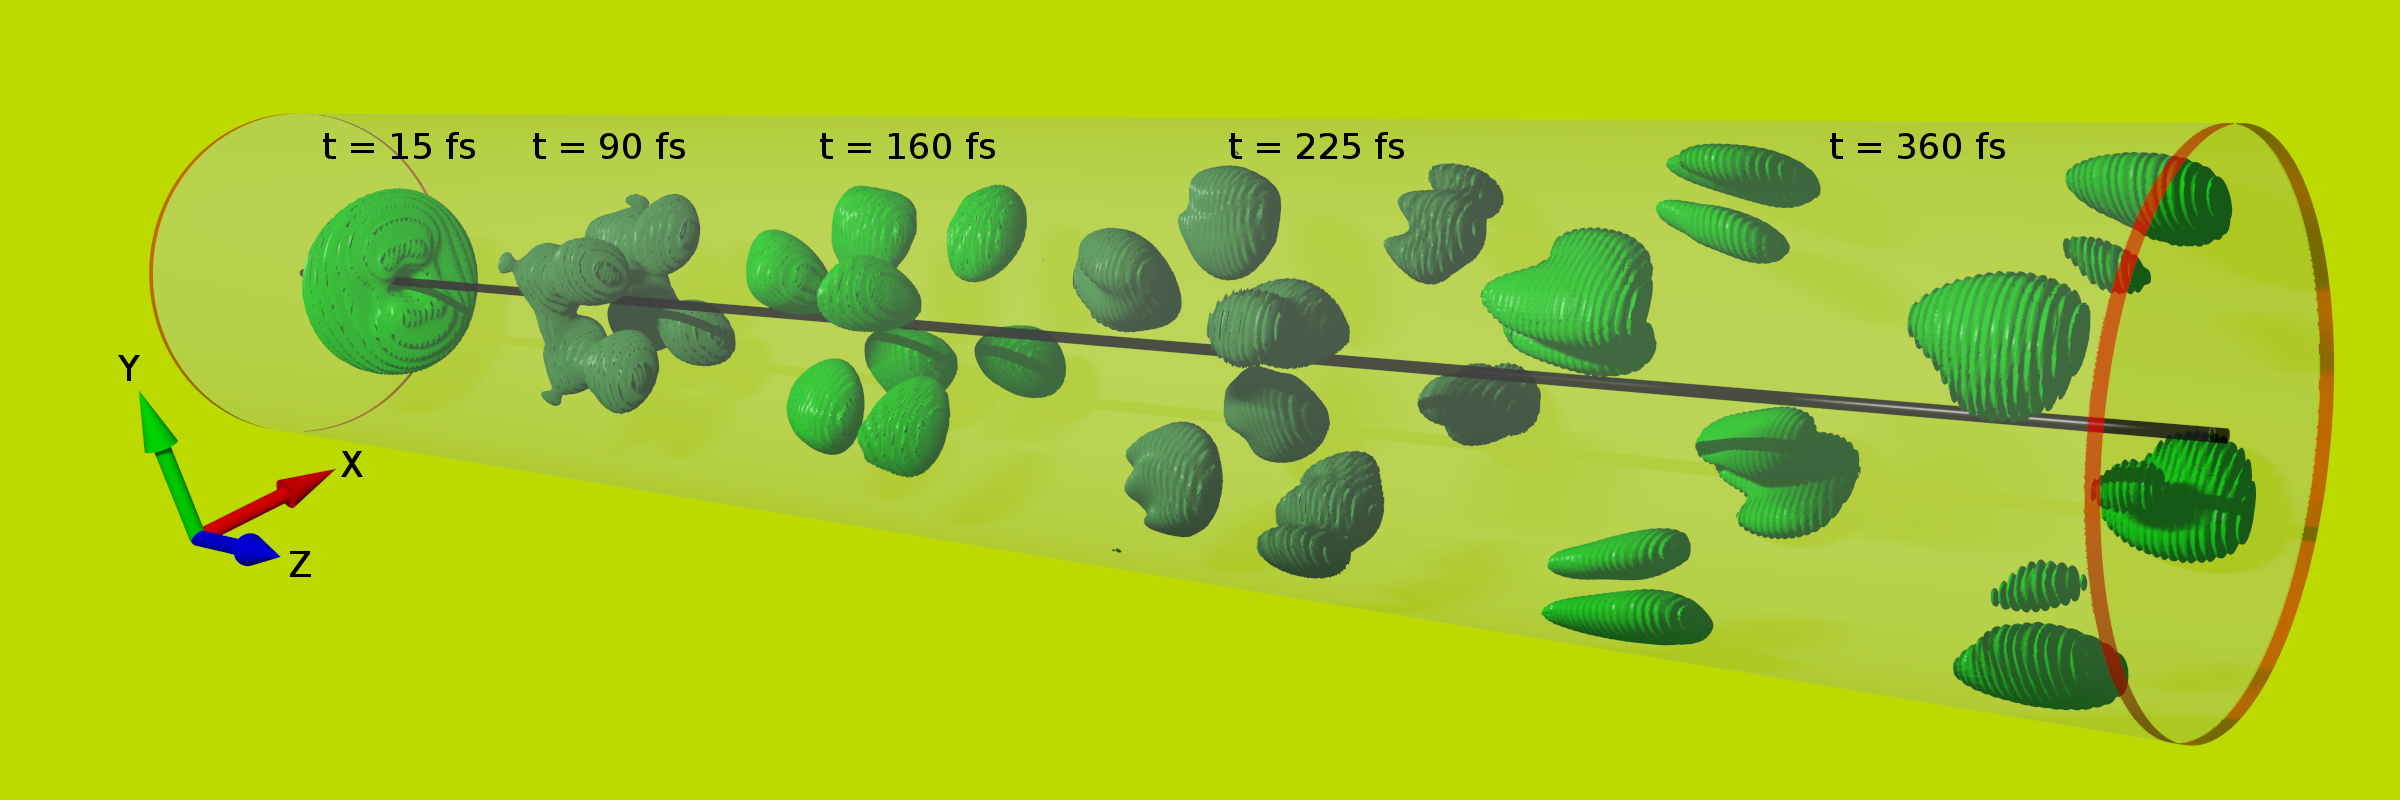
\includegraphics[width=.825\textwidth]{./intensity_gauss_t}
  \caption{Shape of the originally Gaussian pulse at different times after entering the waveguide. Plotted are the isosurfaces where local field amplitude is greater than 5\% of the maximum. At first, the pulse is roughly spherical. Soon a minimum forms at the axis, and the upper and lower parts start overtaking the left and right ones, due to the difference in refraction indexes. The pulse gradually splits into 8 parts, which appears to be a stable configuration. }
 \end{figure}

 \item At room temperature, the stable 8-region configuration only forms in fibres with diameter of at least 10$\mu$m. Thinner fibres do not guide light. 
 \item TODO: Determine the polarization of light in each region. Probably each of the two ranks has different polarization. 
\end{itemize}


\end{block}

\begin{block}{\blockpadding Conclusions}
 \begin{itemize}
  \item A method was developed to model the propagation of light through media with non-uniform fully-anisotropic dielectric tensor, such as liquid crystals
  \item The method was tested to produce correct results for refraction and reflection on an interface, transimitivity of uniform-director liquid crystal between crossed polarizers, and for the photonic band-gap in periodic structures
  \item When applied to a radial-profile liquid crystal waveguide, the method predicts the splitting of a single pulse into eight intensity regions, aligned diagonally around the axis in two ranks
  \item The stability of the 8-region configuration depends on waveguide size and birefringence, hinting at possibility of switching by changing the temperature
 \end{itemize}

\end{block}


 \begin{block}{\blockpadding References}
  \begin{thebibliography}{6}
\bibitem{lasers}M.~Humar, M.~Ravnik, S.~Pajk and I.~Mu\v sevi\v c. Nat. Photonics {\bf 3}, 595 - 600 (2009) 
\bibitem{brasselet}E.~Brasselet~et al. Phys. Rev. Lett. {\bf 103}, 103903 (2005).
\bibitem{taflove}A.~Taflove and S.~C. Hagness. {\em Computational Electrodynamics: The Finite-Difference Time-Domain Method}. Artech House (2005).
\end{thebibliography}

 \end{block}

 \end{column}

\end{columns}

\begin{textblock}{5.5}(0.5,5.75)
 

\end{textblock}

\begin{textblock}{8.5}(6.5,2.5)

\end{textblock}

\end{document}
